\section{Initial Results from Pilot Study}
\label{sec:result}

To further demonstrate the viability of our approach, we present a preliminary analysis of one part of the model, shown in Figure~\ref{fig:model}. The model is based on our pilot data, which included only first-year students from both engineering and non-engineering majors, as shown in Table~\ref{tab:study-participants}. 

\noindent For this analysis, we focused on answering aspects of \ref{itm:rq-behavior} (the impact of daily discrimination on short-term behaviors) and \ref{itm:rq-behavior-size} (the size and length of behavior change). 

\paragraph{Analysis Approach.}
We use hierarchical linear modeling (HLM) for this analysis. HLM is an extension of linear regression for units (\eg individuals, schools, communities) with correlated/common features. %We use a two-level model in which individual participants, who were repeatedly sampled over time, are clustered within themselves.
%HLM allows for flexibility in how change over time is modeled such that these models can fit discontinuous and non-linear changes. Additionally, 
HLM models do not require individuals to report the same number of observations over time and thus can handle an unequal number of observations per person and uneven spacing between observations (\cite{maas2005sufficient}).

Considering the inter-related nature of the variables and their sheer numbers, along with the small number of participants in the pilot study, the behavior features considered as outcomes must be reduced to avoid an excessive number of comparisons that increase the chance of type I error (\eve{define}). 
\begin{wrapfigure}{l}{0.5\textwidth}
\vspace{-1.5em}
    \centering
    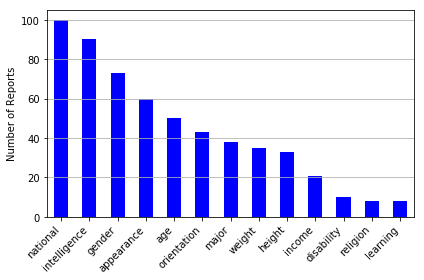
\includegraphics[width=3.3in]{img/discrimination_breakdown.png}
`    \caption[Unfair treatment type breakdown]{Breakdown of \numdiscriminationeventsfinal reports of unfair treatment by type. \textit{National}, \textit{Orientation}, and \textit{Learning} refer to ancestry or national origin, sexual orientation, and learning disability, respectively. See \tbl{tab:study-surveys} for details of all categories. Participants could report multiple types of unfair treatment in each incident report.
}
    \label{fig:data-discrimination-breakdown}
\end{wrapfigure}
Prior to analysis, we used feature selection to reduce the size of the feature space. We selected the top five metrics (when available) for each sensor for further analysis. Much more can be said about analysis, a domain in which PI Mankoff is innovating (\eg \cite{DBLP:conf/huc/EarlyFM16,DBLP:conf/chi/BanovicBCMD16,DBLP:conf/huc/KoehlerBOMD14}). Although not a focus of this proposal, that research and expertise will be leveraged where useful to improve upon this proposed work.

\paragraph{Prevalence of daily discrimination.}
Pilot study data lacked information about race-related discrimination, an approach we corrected in the year one deployment. However, it included discrimination on the basis of a range of other variables, such as ancestry/national origin, intelligence, and gender (the three most common) to religion, learning, and disability (the three least common); see \fig{fig:data-discrimination-breakdown}). Participants reported \numdiscriminationeventsfinal distinct incidents of unfair treatment during the pilot study. \fig{fig:data-discrimination-breakdown} shows the prevalence and breakdown of these reports by category. We found that unfair treatment was more prevalent among women: 73\% of all reports of unfair treatment were reports from women. Contrary to our expectations, unfair treatment was equally prevalent in both engineering and non-engineering majors. \paula{consider saying what all the non students are re disciplines?}


\paragraph{\ref{itm:rq-behavior} Impact of daily discrimination on short-term behavior.} We found short-term impacts of discrimination on mental health and behavior. Discriminatory encounters showed strong (high confidence) relationships with same-day depression and frustration (\textit{p} $<.001$), but no strong relationships with change in positive affect. This is consistent with earlier reports that discrimination is more strongly associated with higher negative but not lower positive states \citep{Schmitt:2014}. Changes in depression and frustration are illustrated in Figure~\ref{fig:reeults-affect-dieoff}.  

We also found a relationship with behavior, particularly behaviors relating to sleep, activities, steps, and phone use \paula{this meaning screen use only or also calls? are the differences in theorized directions?}, which all differed significantly from the baseline on the day of discrimination. This supports our theoretical model, which links discrimination to stress and thus predicts changes in stress-related behaviors. 

\paragraph{\ref{itm:rq-behavior-size} Size and length of short-term behavior change.}

Because we chose to use regression modeling, we could easily quantify the impact of the changes found in ~\ref{itm:rq-behavior}. We found that people walked more (by $\sim$500 steps), had more evening calls ($\sim$1 more), interacted more with their phone in the morning ($\sim$5 more interactions), and spent less time in bed ($\sim$15 minutes less), when they have experienced discrimination in the last day. 

To model the change in impact over time, we examined exposure to discrimination on the day of (day 0) and response variables (health and behavior) on day 1, day 2, etc. and calculated whether there was a significant difference as compared to people who reported no daily discrimination.  We found that discriminatory encounters showed strong (high confidence) relationships with same-day and next-day daily reports of depression and frustration. 

These changes in affect also translated into changes in behavior. To relate them to behavior, we examined six of the most predictive variables found in our analysis. Our results (shown in Figure~\ref{fig:die-off}) demonstrate that most, if not all, of the impact found in our data occurred on  day 0 (day of the discrimination). This effect then declined (\textit{p}-values rise) over the next two days. \paula{is there value in looking at the relationship of chronic discrim or negative events perhaps cumulatively with daily discrim to assess if effects last longer for those with greater prior stress load? this is part of what we have set up in the intro. May decide not to do here but it likely will be important to see trends for those with greater chronicity of stress histories. might add to section below re social support}
%The effect size is also stronger on the day of unfair treatment than the day after (larger $\beta$'s). After that, this distress returns to values similar to those in the control group (people who did not report unfair treatment).

\paragraph{\ref{itm:rq-short-long} Which long-term outcomes are linked to short-term behavior changes?}
Although we lack sufficient longitudinal data to fully analyze this research question (since the pilot data encompasses less than one year of the student experience), we can explore the link between behavior change and mental health. 

We used the same modeling approach to study the impact of mediating factors on the link between short-term behavior change and long-term outcomes. Although the immediate impact of singular instances of unfair treatment faded quickly, people who reported unfair treatment \textit{and} scored lower on social support, reported higher levels of depression at the end of the study ($\beta$ = -0.15, p-value=0.027). This is predicted by the literature  (\eg \cite{Mossakowski:2014}) and aligned with our theoretical model: having social support buffers some of the psychological distress of daily discrimination, and reduces the likelihood that it will impact long-term outcomes.

\begin{figure}
     \centering

% \begin{subfigure}[t]{0.49\textwidth}
% %    \small
%     \centering
%     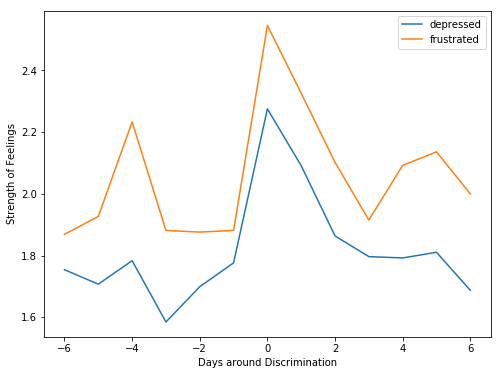
\includegraphics[width=\textwidth]{img/affect-beforeafter.png}
%     \caption[Affect ratings before and after unfair treatment]{Ratings of feeling depressed and frustrated (1: not at all, 5: extremely) 3 days before and 3 days after reports of unfair treatment. The day of unfair treatment is at zero. Note the large peak on the day of the report, which lasts an additional day but then subsides.
%     }
%     \label{fig:reeults-affect-dieoff}
% \end{subfigure}
% % \hfill
% \begin{subfigure}[t]{0.49\textwidth}
%     \centering
    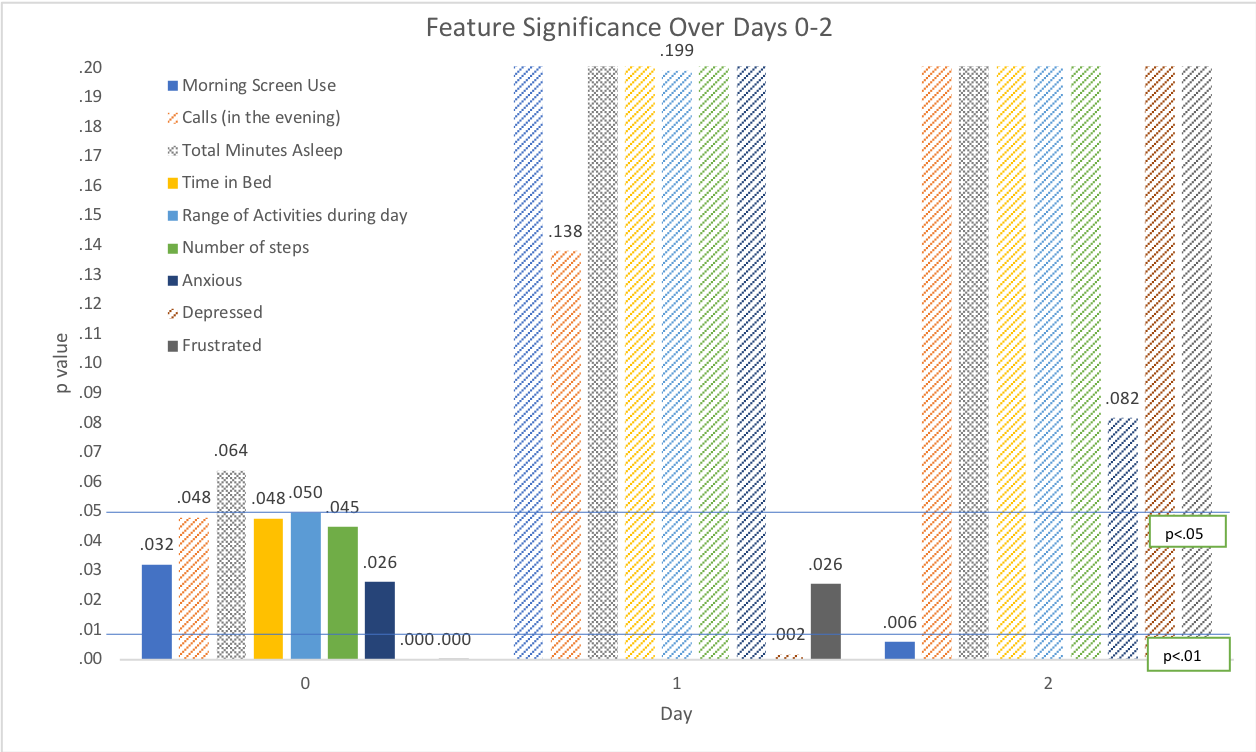
\includegraphics[width=\textwidth]{img/feature-significance}
    \caption[Feature significance over time]{Patterns of feature significance within two days of the discrimination event. The shortest bars represent the highest significance values (\eg Depressed and Frustrated on day 0; Depressed on day 1; Morning screen use on day 2). Most short-term relationships appear on the day of the event and a few on the day after.  Lines are shown at p$<.05$ and p$<.01$.\\ }
    \label{fig:die-off}
% \end{subfigure}

\end{figure}


%\paragraph{Impact of microclimate and other moderators on unfair treatment:} \jen{xx to fill out. There was very old data in the proposal}
%In the chart below, the Y axis shows the percentage of engineers who were at risk on each scale in January (start of study) and June (end of study) of 2018. We choose to focus on engineers in order to compare engineers enrolled in protective micro-climates from their peers who do not share the same protective factors. These micro-climates are the Direct Admit program, in which students are directly admitted to the major and do not have to compete for admission to an engineering department; and the STARS program, which is an onboarding program for first-generation college students, and students from low-income backgrounds and high-poverty high schools in Washington; these students tend to struggle in engineering programs because they  might not be fully prepared for their prerequisite  courses. 

\section{Planned Analyses as Data Is Collected}

Although discrimination is the target of our study, it must be explored in the context of all of the hardships faced by students (and their reactions to the hardships). In our model, this is represented in the form of mediating factors. In our analysis, this also needs to accounted for.

\subsection{\ref{itm:rq-behavior}: The Impact of Discrimination on Short-term Behavior}

 Framing: Which Behaviors? How long? How Severe?
 
 Over the course of the proposed study, we expect to collect approximately 1,800 examples of discrimination from which we can derive information about short term behavior changes. From a statistical and machine learning perspective, this should be more than sufficient to support strong conclusions with respect to \ref{itm:rq-behavior} \ref{itm:rq-behavior-size} and \ref{itm:rq-severity-impact}.

\subsubsection{Measures} The outcome measures we will use to study \ref{itm:rq-behavior} are behaviors, time, and size of behavior change. The first of these outcome measures is by design focused on features of behavior that can be passively captured (as described in \ref{sec:??}, these are extracted from mobile phone sensors). 

\subsection{Analytic approach}
We are proposing to hierarchical multiple regression, which was applied already in our pilot analysis with success. Because of the intersectional nature of our data (i.e. someone may both be a woman, and a person of color; or be engaged in multiple micro-climates), we will need to do repeated analysis focusing on specific sub-populations and factors. 


\subsection{The impact of discrimiantion on long term behavior}
In the case of long term outcomes, our sample size will be approximately 150 (depending on attrition). This is still a sufficient sample size to explore questions such as \ref{itm:rq-short-long}, \ref{itm:rq-which-long} and \ref{itm:rq-severity-long} using outcome measures such as retention in major and GPA and analytic techniques such as regression. 

\subsection{The impact of micro-climates on the overall response to discrimination}
Finally, there is the question of how micro-climates impact students. This is the most exploratory aspect of our study. Micro-climate variations will by the nature of our study only impact small groups of students (such as the \jm{XXFILLIN} students in STARS in our year one cohort). To assess the impact of micro-climates, we will need to move beyond statistical techniques to combine qualitative analysis and quantitative analysis. This will allow us to identify and then look for trends over time using regression to assess how students are impacted, or to identify common themes that might be found outside of those micro-climates, allowing us to increase our sample size.

Although this aspect of the proposed analysis is less well-defined, we are confident that our mixed-methods approach will result in rich data that will be able to inform intervention and suggest valuable future work. This study is part of a much larger effort, as evidenced by the letter of collaboration from the STARS leadership, and we plan to capitalize on that larger momentum to ensure that our work seeds the next steps needed to fully explore the impact of micro-climates. 

The micro-climates we will focus on include STARS, SEEEDS, FIGS, and the Major status. The first is expected based on existing studies of it to have a very positive impact on students, including their likelihood of exposure to discrimination and response to it. The second and third are less rigorous programs, that share certain overlap with STARS. By comparing these we may learn about what aspects of STARS are necessary to its success, and whether those aspects can translate into less time-intensive, more scalable programs effectively. Finally, the major status, specifically competitive effort to join the major (which currently accepts only X\% of students who apply) is likely to have a negative impact on students. 

\subsection{risks}
One challenge for our analysis is the size of our study. Although we plan to pursue funding to expand the sample size, as of this writing, the proposed sample size is approximately 200. Although this is somewhat limiting, we are confident that in the case of short term behavior, our sample will be much larger. This is because, 



While this is smaller than in the case of short term behavior, our expectation based on pilot data is that approximately half of the sample will experience some discrimination, and approximately a quarter will experience repeated discrimination. In addition, based on studies of computer science departments such as the Taulbee report \cite{} it would be normal to expect attrition rates of X\% for men and Y\% for women, which might be attributable to discrimination experiences. 


